\chapter{Обзор литературных источников по динамической симуляции огня}

Моделирование бесформенных объектов, таких как дым, огонь, туман, дымка является
предметом постоянных исследований в области компьютерной графики, поскольку
данные объекты не имеют четко очерченных границ и являются мобильными по своей
природе. Высокая коммерческая ценность данных эффектов в кинематографе и
видеоиграх является двигателем постоянных исследований в данной области.
Наибольший вызов представляет моделирование данных объектов в реальном времени,
где необходимо получить максимально реалистичную симуляцию за время обновления
экранного кадра (60Hz+)~\cite{lec17}.

\section{Эволюция алгоритмов симуляции огня}

\subsection{Истоки. Система частиц}

Пионером компьютерной симуляции огня является Уильям Томас Ривз. В 1983 году в
своей работе он ввел понятие ''система частиц'' в качестве примитива для
моделирования, анимации и рендеринга~\cite{reewes1983}. В фильме ''Звездный путь
2: Гнев Хана'' он смоделировал так называемую ''расширяющуюся стену огня'',
созданную с помощью двухуровневой системы частиц.
(рис.~\ref{fig:reeves_1} и рис.~\ref{fig:reeves_2}).
\begin{figure}[htb]
	\centering
	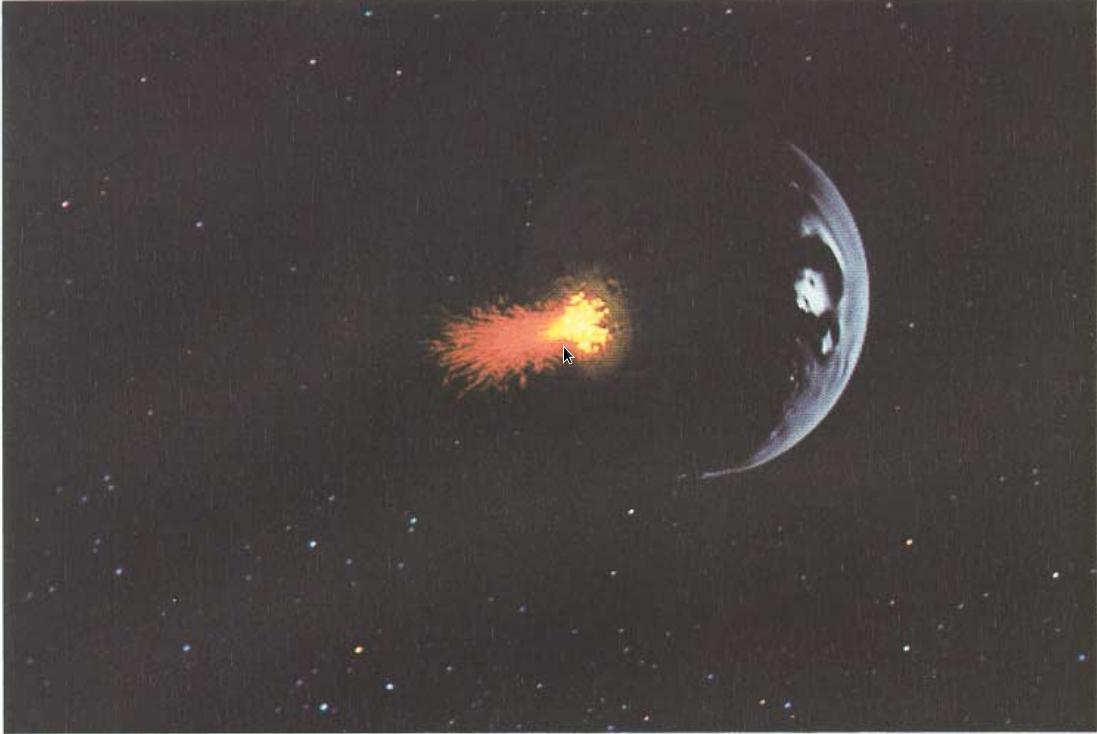
\includegraphics[width=0.7\textwidth]{st2_init}
	\caption{Первоначальный взрыв}%
    \label{fig:reeves_1}
\end{figure}
\begin{figure}[htb]
	\centering
	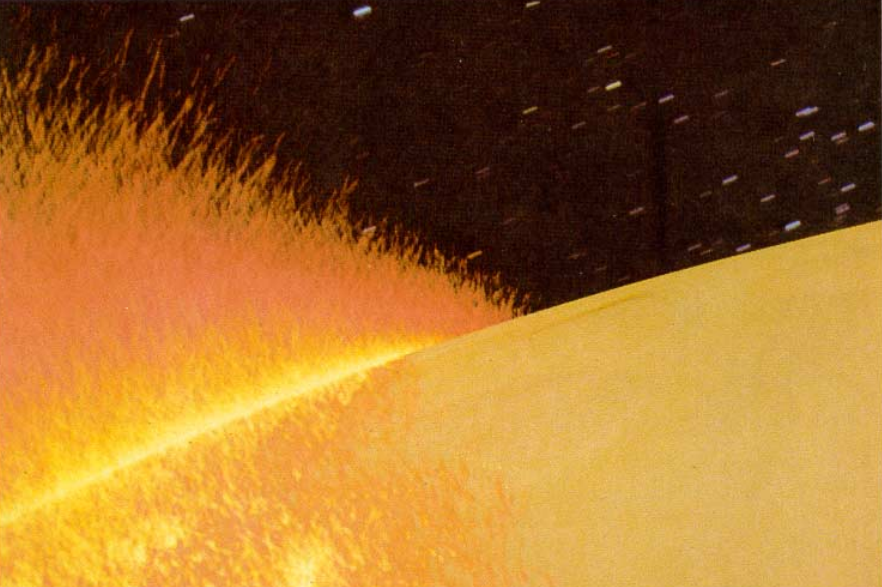
\includegraphics[width=0.7\textwidth]{st2wall}
	\caption{Стена огня вот-вот поглотит камеру}%
    \label{fig:reeves_2}
\end{figure}

Система частиц верхнего уровня находилась в центре взрыва генезис-бомбы, она
генерировала частицы, которые в свою очередь являлись системами частиц. Эти
системы частиц использовались для моделирования взрывов, при которых каждая
такая система частиц вела себя как небольшой вулкан, извергающийся в сторону
распространения взрывной волны и затухающий под воздействием силы гравитации.
Поскольку частицы имеют дискретную природу, для достижения хороших результатов
потребовалось колоссальное количество частиц. Но, поскольку моделирование в
реальном времени не требовалось, это не оказалось проблемой.

\subsection{Оффлайн симуляция}

В данное время наибольшего успеха исследователи добились в нечувствительном к
времени симуляции кинематографе. Несмотря на то, что данная работа нацелена на
компьютерную графику реального времени, необходимо упомянуть несколько работ в
области оффлайн симуляции, поскольку понимание основных идей, заложенных в них,
позволило перенести некоторые из них в область графики реального времени.

В публикации 2002 года Дюк Нгуен и его коллеги представили метод моделирования
огня, полностью основанный на физико-математическом подходе~\cite{nguen2002}. В
симуляции использовались несжимаемые уравнения Навье-Стокса для горячих газов,
это позволило также смоделировать эффект расширения, вызванный испарением, и
эффект текучести поднимающихся дыма и сажи. Демонстрация работы системы
представлена на рисунке~\ref{fig:nguen}.
\begin{figure}[htb]
	\centering
	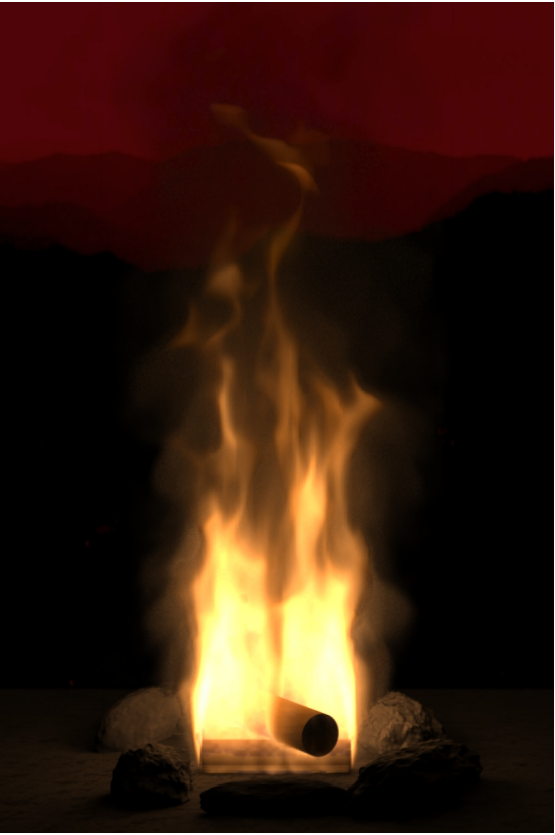
\includegraphics[width=0.3\textwidth]{nguen1}
    \caption{Два горящих полена находятся на земле и являются источником
    топлива. Бревно, лежащее поперек, еще не загорелось, поэтому пламя его
обтекает}%
    \label{fig:nguen}
\end{figure}

Как видно на рисунке, данная симуляция отличается реалистичным
позиционированием и движением газообразных субстанций. Однако данный подход
сложно реализовать в рендеринге реального времени, поскольку необходимо находить
решение большого количества комплексных уравнений за время кадра.

Другой выдающейся работой в этой области является статья Арно
Ламорлетта~\cite{Lamorlette}, опубликованная в 2002 году. В данной работе автор
представил совершенно другой подход в области оффлайн симуляции огня. Данный
подход был использован в мультфильме Шрек студии Dreamworks
(рис.~\ref{fig:shrek}).
\begin{figure}[htb]
	\centering
	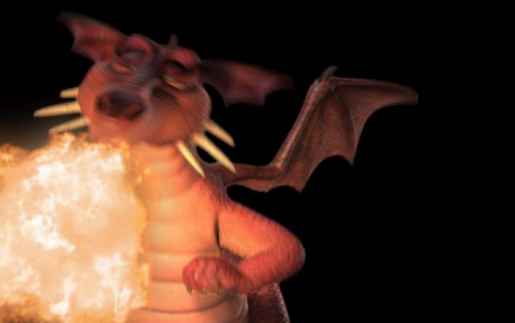
\includegraphics[width=0.7\textwidth]{shrek}
    \caption{Кадр из мультфильма Шрек}%
    \label{fig:shrek}
\end{figure}
В симуляции Ламорлетта фокус с реалистичности смещен в сторону на эстецизма,
управляемости и гибкости. Автор руководствовался идеей, что имея задачу
предоставить инструмент для художественного и поведенческого контроля, будет
крайне сложно достичь поставленной цели полагаясь строго на физические
уравнения.

В 2009 году Кристофер Хорват и Вилли Гейгер представили инновационную комбинацию
симуляции с помощью крупной решетки частиц и тонко настроенных
визуально-ориентированных улучшений симуляции, рассчитываемых на графическом
процессоре (ГП)~\cite{Stock2008}. Полученные изображения
имеют поразительную детализацию и могут быть легко интегрированы в
кинематографические фотоснимки (рис.~\ref{fig:gpu2008}).
\begin{figure}[htb]
	\centering
	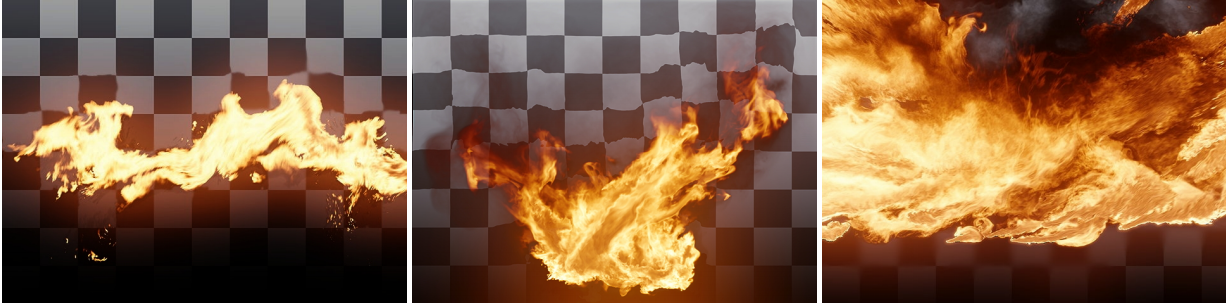
\includegraphics[width=\textwidth]{gpu2008}
	\caption{Три различных кадра симуляции огня. Быстро движущийся огненный
	шар с искрами. Извивающийся костер. Плотная стена дыма и огня.}%
    \label{fig:gpu2008}
\end{figure}
Данная техника улучшения симуляции использует особенности и ограничения
зрительного восприятия, а также особенности концентрации внимания зрителя.
Множество независимых ГП используются для быстрого увеличения качества
изображения, что позволяет достичь очень высокого разрешения.

В статье~\cite{suspendedExplosions} автор описывает метод анимации
приостановленных взрывов. Данный метод использует несжимаемую модель жидкостей
для расчета движения воздуха и горючих газов. Горение смоделировано с помощью
частиц и систем жидкостей. Полученная система позволяет генерировать кадр взрыва
всего за несколько секунд. Сравнение кадра, созданного системой, с реальным
взрывом приведено на рисунке~\ref{fig:explosions}.
\begin{figure}[htb]
	\centering
	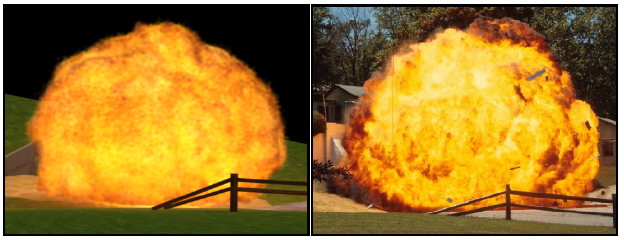
\includegraphics[width=0.7\textwidth]{explosions}
	\caption{Сравнение взрыва из симулятора с фотографией взрыва в угольной
    шахте}%
    \label{fig:explosions}
\end{figure}
Принципы, заложенные в данной публикации в дальнейшем были доработаны и
реализованы в публикации~\cite{VortexExplosions}.

Одной из наиболее эффектных сцен с использованием симуляции огня можно назвать
сцену сожжения Озерного города в фильме ''Хоббит: Битва пяти воинств''
(рис.~\ref{fig:hobbit}).
\begin{figure}[htb]
    \centering
    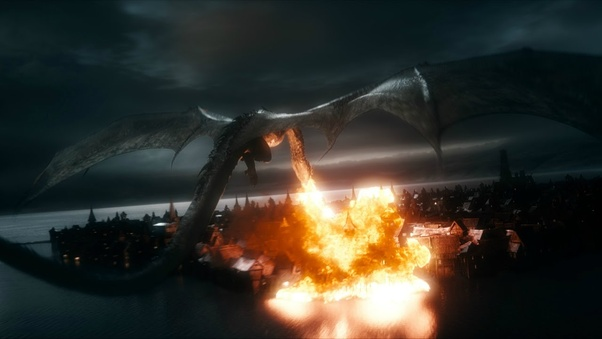
\includegraphics[width=\textwidth]{hobbit}
    \caption{Сцена сожжения Озерного города}%
    \label{fig:hobbit}
\end{figure}
Обзор техник, использованных в фильме приведен в
презентации~\cite{hobbitSlides}. Взмахи крыльев Смауга приводили в движение
симуляцию воздушных потоков. Симуляция воздушных потоков в свою очередь влияла
на симуляцию огня, которая оказывала влияние на детализированное разрушение
окружения с помощью физики твердого тела. Физика разрушения зданий
взаимодействовала с симуляцией воздушных потоков, вызывая подъем дыма и пара.
Когда дракон выдыхал огонь, происходил расчет всех вышеописанных действий.

\subsection{Онлайн симуляция}

Трехмерный огонь, моделируемый в реальном времени, находит свое применение в
интерактивных приложениях. Среди интерактивных приложений можно выделить
компьютерные игры, в которых необходимость показывать взрывы появилась
практически с самого момента их появления (рис.~\ref{fig:earlyGames}).
\begin{figure}[htb]
    \centering
    \subfloat[\small{Огонь создан с помощью заранее нарисованного ядра
	битовой карты, которое окружают анимированные
времени частицы}]{{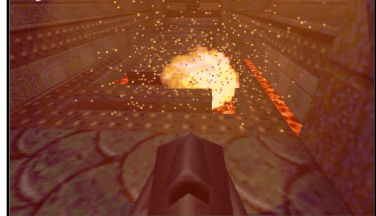
\includegraphics[height=4.0cm]{doom_splat} }}
    \qquad
    \subfloat[\small{Объемный факел, созданный из непрозрачных полигонов}]
    {{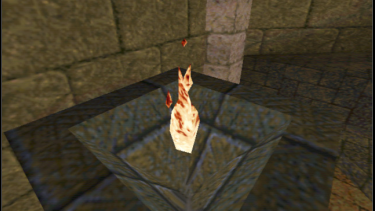
\includegraphics[height=4.0cm]{doom_torch} }}
    \caption{Скриншоты из Quake (1996)}%
    \label{fig:earlyGames}%
\end{figure}

Компьютерные игры являются основными потребителями графических компьютерных
анимаций огня. Однако это стало возможным лишь пару десятилетий назад. С тех пор
скорость аппаратного обеспечения для рендеринга время росла экспоненциально,
открывая возможности для все более и более детализированных эффектов. К
сожалению, поскольку игры зачастую являются проприетарными по своей природе,
литературных источников по алгоритмам, используемых в играх крайне
мало~\cite{capstone}.

В 2014 году была представлена система NVIDIA FlameWorks~\cite{Green2014}. Данная
система позволяет добавлять реалистичный огонь, дым и эффекты взрывов в игры.
Данная система совмещает передовую симуляцию жидкостей на основе решетки вместе
с эффективной системой объемного рендеринга. Все компоненты системы
оптимизировано для работы в реальном времени. Все вычисления выполняются на ГП с
помощью DirectX 11. На рисунке~\ref{fig:FlameWorks} представлен кадры из
демонстрационного ролика.
\begin{figure}[htb]
	\centering
	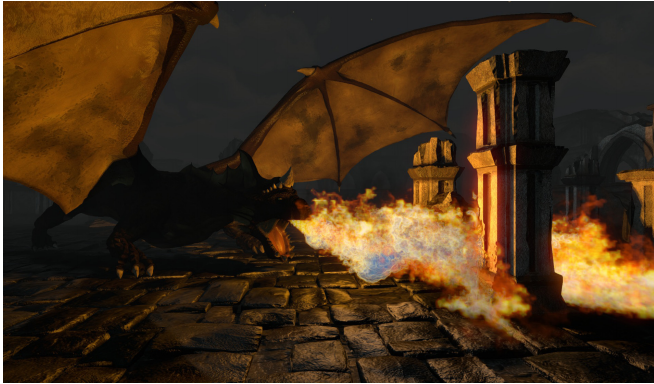
\includegraphics[width=\textwidth]{green2014}
	\caption{Демонстрация работы NVIDIA FlameWorks}%
    \label{fig:FlameWorks}
\end{figure}
В данном ролике использовалась воксельная решетка размерами $512 \times 256
\times 256$ вокселей, каждый кадр обновлялось около 32 миллионов вокселей.
Данная симуляция работала с частотой выше 30 кадров в секунду на GeForce Titan.

В работе~\cite{Somasekaran2005UsingPS} автор подробно описывает создание
симулятора на основе систем частиц. Для структуризации объектов в системе автор
использовал четырехуровневую иерархию (частица, эмиттер, семейство эмиттеров,
менеджер эмиттеров). Это позволило ему создавать сложное пламя, состоящее из
нескольких разнородных источников с различной интенсивностью. Для моделирования
автор использовал совместно идеи из термодинамики и идеи из теории роевого
поведения. Использование алгоритма косяка птиц позволило добиться анимации языка
пламени как единого целого.

Юрий Ванзин в своей диссертации~\cite{Vanzine2007RealisticRR} использовал
сплайны для моделирования языков огня. Автор использовал частицы для расчета
анимации, которые в дальнейшем использовались в качестве скелета для сплайнов.
Для расчета макро-движения огня автор использовал: скорость эмиттера, поля
ветров, диффузионное смещение и термальную текучесть. В результате работы, у
автора получилось создать полноценный фреймворк для рендеринга огня на основе
игрового движка Irrlicht.

В работе~\cite{turbulence} работе представлена система, которая предназначена
для использования 3D-художниками. Пользователь может задать форму пламени на
различных этапах в виде рисунка. Система производит расчет промежуточных кадров
и позволяет экспортировать результаты для рендеринга в графических редакторах.
Данный метод использует в качестве примитива моделирования частицы, рендеринг
осуществляется с помощью сплайнов. Данный алгоритм развивает идеи, предложенные
ранее в~\cite{Vanzine2007RealisticRR}. Для управления анимацией огня авторы
используют четыре вида полей ветров (рис.~\ref{fig:windFields}):
\begin{itemize}
    \item равномерное;
    \item вихревое;
    \item поле-источник;
    \item поле-сток.
\end{itemize}
\begin{figure}[htb]
	\centering
	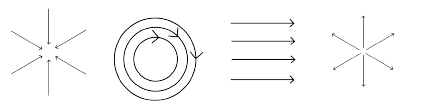
\includegraphics[width=\textwidth]{windFields}
    \caption{Различные виды полей ветров}%
    \label{fig:windFields}
\end{figure}

Интересный подход к проблеме был предложен в~\cite{Lee2011ThreeDF}. Схема
системы приведена на рисунке~\ref{fig:apsipa}
\begin{figure}[htb]
	\centering
	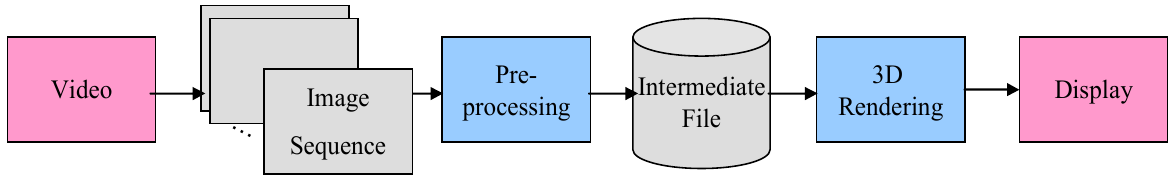
\includegraphics[width=\textwidth]{apsipa}
    \caption{Схема системы из~\cite{Lee2011ThreeDF}}%
    \label{fig:apsipa}
\end{figure}
На первом этапе метода происходит сбор информации из видео с помощью алгоритмов
цифровой обработки изображений. Из полученных данных происходит извлечение
признаков для обучения модели. Результат полученный с помощью обученной модели
используется совместно с процедурными методами для рендеринга анимации огня.
Результаты работы системы выглядят более реалистично по сравнению с
традиционными методами, а способность взаимодействовать с окружением находится
примерно на уровне других методов реконструкции огня.

В статье~\cite{Zhao2003VoxelsOF}, описывается симуляция огня с помощью вокселей.
Авторами предложены алгоритмы распространения огня и поглощения огнем горючих
предметов. Данные алгоритмы предназначены для работы на объемных наборах данных.
Языки пламени в предложенном методе создаются на основе метода решеточных
уравнений Больцмана (LBM). Полученная авторами система позволяет моделировать
распространение огня, горение объектов. Работа системы продемонстрирована на
рисунке~\ref{fig:voxelFire}.
\begin{figure}[htb]
	\centering
	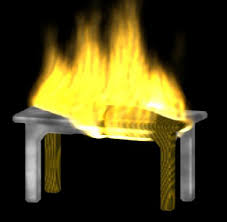
\includegraphics{voxels_on_fire}
    \caption{Воксельное пламя}%
    \label{fig:voxelFire}
\end{figure}
На рисунке изображен объемный стол. Внутренняя основа из негорючего металла
открывается по мере того, как сгорает внешний слой из дерева.

Статья~\cite{Lyes2013FireAF} описывает методы ускорения симуляции огня с помощью
технологий параллельных вычисления CUDA, также авторы исследовали поведение
системы с различными примитивами рендеринга (точки, треугольники, текстуры).
Полученные результаты показывают в среднем улучшение на 10\% при использовании
параллельного кода на CUDA\@. Рендеринг с помощью точек показал наивысшую
производительности, однако рендеринг с помощью текстур показал лучшие визуальные
результаты. По результатам опытов было найдено оптимальное ядро $128 \times
128$, что соответствует 16384 частицам в системе.

В работе~\cite{MeshesOnFire} метод анимации огня на многогранных поверхностях.
Для расчетов в данном методе используются простая геодезия на мешах, скорость,
зависящая от внешнего ветра или сил, угол наклона, и другие атрибуты. В отличие
от предыдущих методов, данный метод позволяет выполнять отложенный адаптивный
расчет фронта огня, метод также обрабатывает точки стыка, объединение фронтов и
поддерживает удаленное возгорание. Все эти приемы помогают достаточно
реалистично отобразить поведение реального огня.

Авторы работы~\cite{FireSplats} предлагают в своей статье использовать
текстурные сплэты в качестве базового примитива рендеринга. Для реализации
взаимодействия огня с ветром и окружающими объектами авторы использовали простую
линейную LBM\@. Результаты симуляции можно увидеть на
рисунке~\ref{fig:textureSplats}.
\begin{figure}[htb]
	\centering
    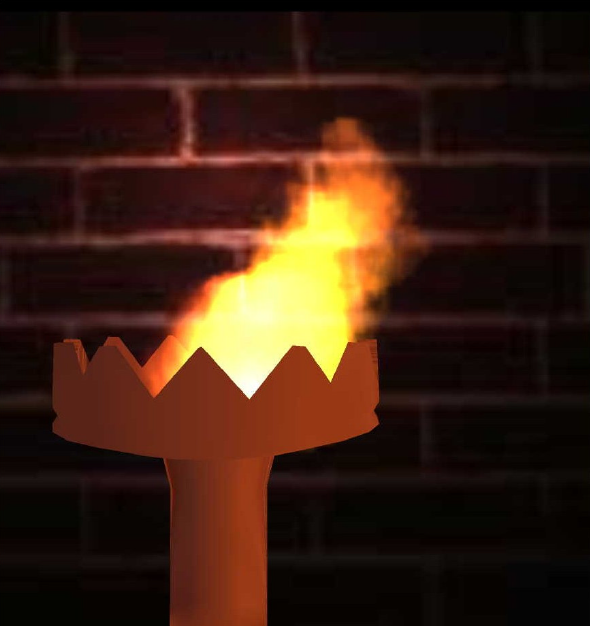
\includegraphics[width=0.5\textwidth]{textureSplats}
    \caption{Симуляция огня в системе~\cite{FireSplats}}%
    \label{fig:textureSplats}
\end{figure}
Полученная ими система имеет следующие преимущества:
\begin{enumerate}
    \item Турбулентное поведение огня может быть выражено с помощью текстурных
        сплэтов.
    \item Расчеты LBM могут быть выполнены на ГП.
\end{enumerate}

В недавней статье~\cite{Jo2019LatticeBoltzmannAE} авторы предлагают новый
гибридный метод симуляции для моделирования процессов горения твердого топлива.
Авторы создали гибридную систему на основе метода решеточных уравнений Больцмана
и уравнений Навье-Стокса (решетка Эйлера). В данной работе показано, что
вычислитель на основе уравнений Навье-Стокса может быть использован для расчета
участков огня, находящихся в воздухе. Для расчета поведения огня внутри и на
поверхности твердых тел авторы рекомендуют использовать LBM\@.

Авторы работы~\cite{Sato2012ADA} предлагают простой и эффективный подход для
создания высокодетализированных 3D анимаций из низкодетализированных симуляций
на основе физики жидкостей. Создатели алгоритма используют заранее рассчитанную
базу полей скорости, полученных из двумерных симуляций на основе физики
жидкостей. Во время работы программы выполняется низкодетализированная 3D
симуляция, поля скоростей симуляции каждый шаг апроксимируются с помощью
линейной комбинации заранее рассчитанных полей. С помощью такого метода
пользователи могут разрабатывать низкодетализированные анимации и добавлять к
ним детали на завершающих этапах (рис.~\ref{fig:highRes}).
\begin{figure}[htb]
	\centering
    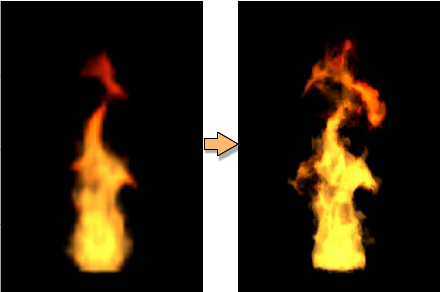
\includegraphics[width=0.5\textwidth]{highRes}
    \caption{Преобразование огня с разрешением $32 \times 32 \times 64$ точек в
    огонь с разрешением $128 \times 128 \times 256$ точек}%
    \label{fig:highRes}
\end{figure}

В статье~\cite{MultiView} авторы представляют один из методов томографической
реконструкции огня. Структура метода представлена на рисунке~\ref{fig:fireReco}.
\begin{figure}[htb]
	\centering
    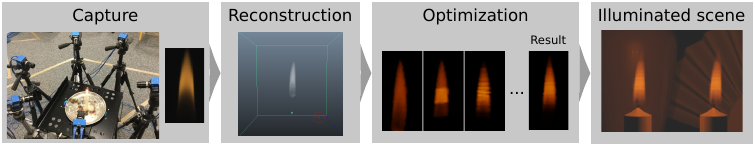
\includegraphics[width=\textwidth]{fireReco}
    \caption{Стадии метода реконструкции огня из~\cite{MultiView}}%
    \label{fig:fireReco}
\end{figure}
С помощью RGB камер происходит запись анимации реального огня. Далее на стадии
реконструкции происходит расчет плотности объема занимаемого огнем. На стадии
оптимизации происходит вычисление температур участков пламени и расчет полей
плотности горючего. Рассчитанные модели в дальнейшем могут быть использованы для
создания реалистичного освещения в виртуальных сценах. Отличием данной работы от
предыдущих решений является то что созданный огонь дает реалистичное освещение
сцены без необходимости искусственного создания дополнительных источников
освещения.

В работе~\cite{DiffusionProcesses} приводится исчерпывающее описание
использования диффузионных процессов для симуляции газообразных феноменов.
Авторы представили простую модель анимации и распространения огня, также ими
была разработана эффективная реализация алгоритма глобального освещения в
присутствии газов и огня. В отличие от предыдущих работ в данной области, данная
работа предоставляет дополнительный уровень контроля пользователю над развитием
газообразного феномена. Такие параметры, как позиционирование полей ветров, их
размер и магнитуда могут быть изменены в режиме реального времени.

Интересная термодинамическая модель пламени предложена
в~\cite{InteractiveSimulation}. Авторам удалось создать быструю интерактивную
модель симуляции огня, предоставляющую высокий уровень реалистичности. В данной
системе процесс горения симулируется с помощью поглощения топлива и окисляющих
газов в каждой ячейке сетки сцены. Процесс горения вызывает выделение тепла,
распределение и распространение которого моделируется в системе. Процесс
распространения тепла создает конвекционные потоки в воздухе, придавая
соответствующую форму пламени. Кроме моделирования распространения тепла, в
данной системе также симулируется процесс распространения огня и процессы
самовозгарания твердотопливного горючего.

Использование симуляции огня для создание стилизованных арт-работ приведено в
диссертации~\cite{Bangalore2012ATF}. Автору удалось создать простую для
использования художниками систему. Пользователи могут создавать и анимировать
контрольные линии в привычных им пакетах и импортировать результаты в систему.
Симулятор использует вычислитель для уравнений стационарных жидкостей и
показывает довольно быструю работу на относительно низких разрешениях (100
вокселей на слайд), что позволяет выполнять визуализацию в реальном времени с
помощью OpenGL~\@. Результаты работы системы представлены на
рисунке~\ref{fig:artRenderer}.
\begin{figure}[htb]
	\centering
    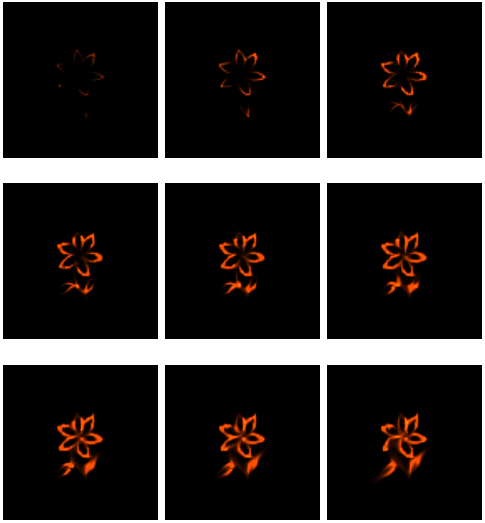
\includegraphics[width=0.6\textwidth]{artRenderer}
    \caption{Рендеринг огненного цветка}%
    \label{fig:artRenderer}
\end{figure}

В статье~\cite{ForGames} в представлена простая и быстрая
реализация вычислителя динамики жидкостей для игровых движков. Данный инструмент
основан на уравнениях Навье-Стокса для расчета поведения жидкостей. Вычислитель,
предложенный в работе в первую очередь нацелен на визуальное качество. Авторы
демонстрирует простоту их реализации, предоставляя в публикации полный код
симулятора на языке Си. Предложенный алгоритм может использоваться для расчета
сеток разумного размера в реальном времени, используя для этого обычный
персональный компьютер.

В работе~\cite{NaturalPhenomena} приведено описание эффективных методов для
создания реалистичных изображений природных феноменов. В данной работе приведены
алгоритмы и уравнения для создания дыма, облаков, неба. В качестве примитива
симуляции выбраны частицы. Описанные в статье методы могут быть использованы для
получения фотореалистичных изображений.

В презентации~\cite{RealTimeNVIDIA} приводится хороший обзор истории симуляции
огня и состояния проблемы на сегодняшний день. Авторы приводят код простого
вычислителя давления жидкостей на CUDA\@. Также авторы дают ряд подсказок по
симуляции огня, позволяющих добиться максимальной реалистичности симуляции.
Среди этих советов можно особенно выделить следующие:
\begin{enumerate}
    \item Постобработка крайне важна. С помощью таких приемов как размытие в
        движении и свечение объектов (рис.~\ref{fig:GlowEffect}) можно лучше
        доносить зрителю информацию о температуре.
    \begin{figure}[htb]
        \centering
        \subfloat[\small{Без эффекта
        свечения}]{{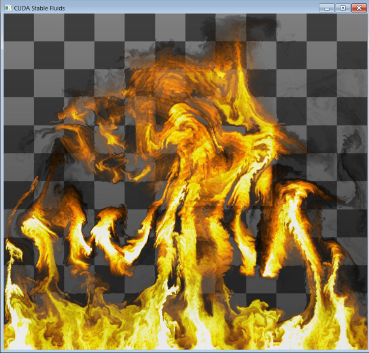
\includegraphics[width=7.5cm]{noGlow} }}
        \qquad
        \subfloat[\small{С эффектом свечения}]
        {{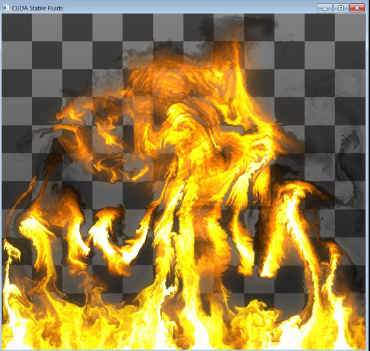
\includegraphics[width=7.5cm]{Glow} }}
        \caption{Влияния эффекта свечения на симуляцию огня}%
        \label{fig:GlowEffect}%
    \end{figure}
    \item Добавление шумов. Добавление процедурного шума позволяет создать
        эффект турбулентности и увеличить реалистичность.
    \item Искры. Для добавления искр авторы советуют использовать
        четырехугольники, растянутые от прошлой позиции до текущей. Для этого
        рекомендуется использовать геометрический шейдер.
\end{enumerate}

Авторы статьи~\cite{RealTimeVolumetric} представили в 2007 году метод для
генерации процедурного объемного огня в режиме реального времени
(рис.~\ref{fig:proceduralFire}).
\begin{figure}[htb]
	\centering
    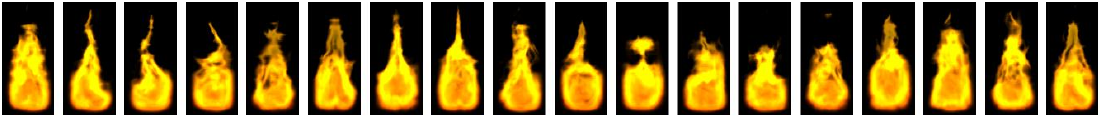
\includegraphics[width=\textwidth]{proceduralFire}
    \caption{Процедурный шум используется для придания каждому огню уникального
    вида}%
    \label{fig:proceduralFire}
\end{figure}
С помощью комбинации кривообразной объемной свободной деформации, рендеринга с
использованием аппаратного ускорения и М-шума авторам удалось создать
подрагивающий огонь с уникальной анимацией. Данный метод поддерживает
эффективное обнаружение коллизий, что, вкупе с хорошо спроектированной системой
частиц позволяет, позволяет добиться двухстороннего интерактивного
взаимодействия между огнем и окружающей его средой.

В статье~\cite{SpringMass} представлен метод симуляции трехмерного огня в режиме
реального времени (рис.~\ref{fig:campFire}).
\begin{figure}[htb]
	\centering
    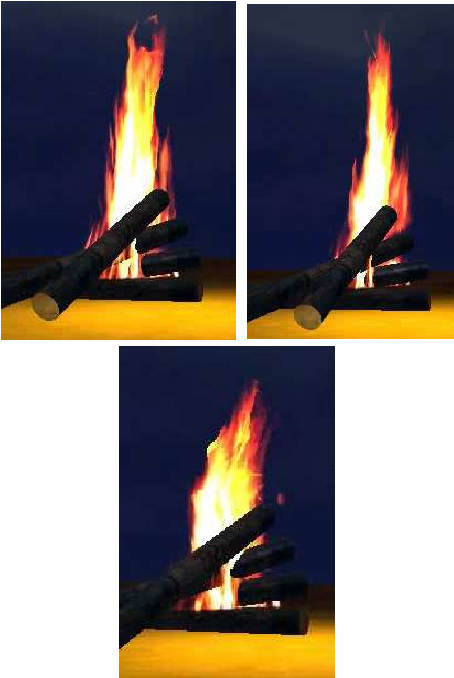
\includegraphics[width=0.4\textwidth]{campFire}
    \caption{Костер, созданный с помощью 8 различных текстур}%
    \label{fig:campFire}
\end{figure}
Идею данного метода авторы взяли из старого механического приема под названием
''шелковый факел''. Авторы выполняли моделирование кинематики огня с помощью
уравнений гармонических колебаний, а турбулентность и визуальную динамику с
помощью последовательностей текстур с различной прозрачностью. Текстуры
определялись скоростью топливных газов.

\section{Обзор и классификация алгоритмов симуляции огня}

В предыдущих разделах было описано множество различных методов симуляции огня,
однако, можно обобщить данные методы и выделить отдельные классы. Различные
методы применяемые при симуляции огня можно разделить на следующие
группы:
\begin{itemize}
	\item текстурный маппинг;
	\item системы частиц;
	\item физико-математические методы;
	\item клеточные автоматы;
	\item томографическая реконструкция и др.
\end{itemize}

В работе~\cite{realistic_sim} представлен детальный обзор различных техник для
создания реалистичной симуляции огня. В данной работе проведен сравнительный
анализ нескольких техник симуляции огня, включая симуляцию с помощью вокселей и
симуляцию с помощью стационарных жидкостей. Приведено кратное описание каждой
техники, с описанием их преимуществ и недостатков.

В 2011 году Чжао Хуэй и его коллеги представили статью~\cite{survey}, авторы
проанализировали большое количество методов симуляции огня и смогли выдвинуть
свою классификацию методов. Авторами был проведен анализ наиболее популярных
методов по следующим критериям:
\begin{itemize}
	\item применимость в реальном времени;
	\item степень реалистичности;
	\item пространственно-временная сложность;
	\item настраиваемость;
	\item интерактивность.
\end{itemize}

Результаты данного исследования можно увидеть в таблице~\ref{table:algoAnalsysis}.
\begin{table}[htb]
    \caption{Сравнение производительности различных методов симуляции огня}
    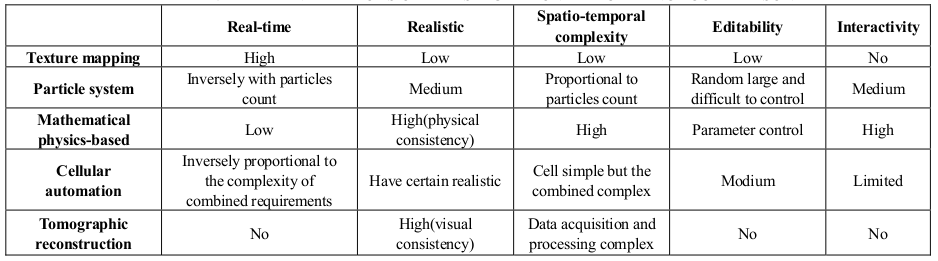
\includegraphics[width=\textwidth]{simulation_methods}%
    \label{table:algoAnalsysis}
\end{table}

В процессе исследования работ по симуляции огня, авторы смогли выделить
следующие проблемы:
\begin{enumerate}
    \item Системы частиц демонстрирует определенный уровень детализации огненной
        сцены, особенно удачно они отражают случайные изменения в огне. Однако,
        их поведение слишком непредсказуемо, чтобы достичь точного отображения
        огня.
    \item Математические методы, основанные на физике, предоставляют большие
        преимущества в реалистичности, настраиваемости и интерактивности, но они
        с трудом подходят к применению в реальном времени.
    \item Метод клеточных автоматов лучше всего подходит для моделирования
        распространения огня, поскольку пространственно-временная сложность
        данного метода сильно ограниченна из-за необходимости комбинации клеток.
    \item Методы томографической реконструкции по изображению позволяют
        генерировать точные анимации огня, которые могут быть отрисованы в
        произвольных позициях. Данные методы не могут предоставить широкие
        возможности по настраиваемости и интерактивности. Вдобавок к этому, цены
        на оборудование для сбора данных крайне высоки.
\end{enumerate}

\textbf{Выводы по главе 1:}
\addcontentsline{toc}{section}{Выводы по главе 1}
\begin{enumerate}
    \item При выборе алгоритма для динамической симуляции необходимо найти
        баланс между реалистичностью симуляции и скоростью симуляции. Частота
        кадров не должна падать ниже заданного минимального порога.
    \item Большую роль в создании реалистичной симуляции играет постобработка.
        Такие вещи, как добавление шумов и размытия позволяют существенно
        увеличить реализм сцены.
    \item Моделирование огня с помощью системы частиц до сих пор является
        наиболее популярным методом, который позволяет обеспечить средний
        уровень реалистичности, но при небольшом количестве частиц обеспечивает
        высокую скорость симуляции. Данный метод будет использован для
        моделирования частиц в рамках диссертации.
    \item Использование алгоритмов из области физики, в особенности
        термодинамики позволяет создавать реалистичные симуляции. Некоторые из
        физических алгоритмов хорошо показали себя на практике и будут
        использованы для создания симулятора в рамках диссертации.
\end{enumerate}
